\documentclass[11pt]{article}
\usepackage[a4paper, margin=1in]{geometry}
\usepackage{amsmath}
\usepackage{graphicx}
\usepackage{hyperref}
\usepackage{enumitem}
\usepackage{titlesec}
\usepackage{microtype}
\linespread{1.1}
\titleformat{\section}{\large\bfseries}{\thesection.}{1em}{}
\titleformat{\subsection}{\normalsize\bfseries}{\thesubsection.}{1em}{}

\title{\textbf{Reinforcement Learning: Concepts, Techniques, and Applications to Large Language Models}}
\author{Sabína Ságová}
\date{}

\begin{document}

\maketitle

\section*{Abstract}
Reinforcement Learning (RL) is a foundational area of machine learning that empowers agents to make sequential decisions through trial-and-error interactions with an environment. Unlike supervised learning, which relies on labeled datasets, RL agents learn optimal behavior by maximizing cumulative reward signals. This learning paradigm is particularly powerful in domains involving uncertainty and long-term planning, such as robotics, control systems, and increasingly, the training and alignment of large language models (LLMs) like ChatGPT. This paper outlines core RL principles, summarizes key algorithmic approaches, and explores how RL---particularly Reinforcement Learning from Human Feedback (RLHF)---is reshaping the behavior of LLMs.

\section{Introduction}
Reinforcement Learning offers a framework for learning via interaction, where an agent learns to maximize a long-term reward signal through feedback from the environment. It has gained increasing relevance in generative AI, where aligning outputs with human expectations remains a critical challenge. RL provides a mechanism for continuous, feedback-driven refinement of model behavior.

\section{Theoretical Foundations}
At the core of RL lies the \textit{Markov Decision Process (MDP)}, defined by:
\begin{itemize}[noitemsep]
    \item A set of states $S$
    \item A set of actions $A$
    \item A transition probability $p(s', r \mid s, a)$
    \item A reward function $R$
    \item A discount factor $\gamma \in [0,1]$
\end{itemize}

At each timestep $t$, the agent observes state $S_t$, chooses action $A_t$, receives reward $R_{t+1}$, and transitions to state $S_{t+1}$, where future outcomes depend only on the current state and action---the Markov property.

\begin{figure}[h]
    \centering
    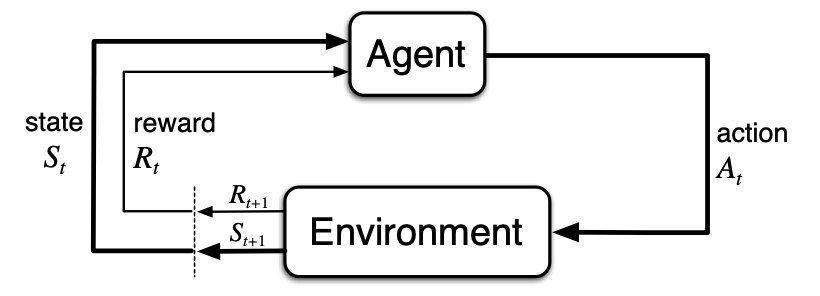
\includegraphics[width=0.7\textwidth]{mdp.png}
    \caption{The agent–environment interaction in a Markov decision process.}
    \label{fig:mdp}
\end{figure} 
\newpage
\section{Key Algorithms}
Several families of RL algorithms are foundational:
\begin{itemize}[noitemsep]
    \item \textbf{Dynamic Programming}: Requires full environment knowledge (e.g., value iteration).
    \item \textbf{Monte Carlo Methods}: Learn from episodes, suitable for unknown environments.
    \item \textbf{Temporal Difference (TD) Learning}: Combines DP and Monte Carlo; includes SARSA and Q-Learning.
    \item \textbf{Policy Gradient Methods}: Optimize policies directly, especially useful in continuous spaces.
    \item \textbf{Deep Reinforcement Learning (DRL)}: Uses neural networks to approximate policies or value functions (e.g., DQN, PPO).
\end{itemize}

\section{Reinforcement Learning in LLMs}
Reinforcement Learning has become central to training aligned, safe large language models. Traditional supervised training cannot always capture the complexity of human preferences. This gap is addressed by \textbf{Reinforcement Learning from Human Feedback (RLHF)}.

The RLHF pipeline typically involves:
\begin{enumerate}[noitemsep]
    \item Generating multiple outputs from the model.
    \item Ranking or scoring them using human evaluators.
    \item Training a reward model to predict preference scores.
    \item Fine-tuning the model via Proximal Policy Optimization (PPO) to maximize the predicted reward.
\end{enumerate}

\textit{Example:} A prompt such as ``Explain black holes to a 12-year-old'' may yield several completions. Human annotators rank them based on clarity and tone. The model then learns to produce outputs similar to the top-ranked completions.

\section{Recent Developments}
The Kimi k1.5 model (Kimi Team, 2025) exemplifies the practical benefits of reinforcement learning for language models. By combining supervised pretraining with reward-based fine-tuning, Kimi k1.5 improves response relevance and achieves state-of-the-art reasoning performance across multiple benchmarks. Its simplified, scalable RL approach—eschewing complex elements like value functions and Monte Carlo tree search—demonstrates how reinforcement learning can be effectively applied to real-world LLM use cases while maintaining robustness.
\section{Conclusion}
Reinforcement Learning, and particularly RLHF, provides a critical toolkit for aligning LLMs with human values and expectations. As generative models evolve in capability and scope, RL will remain essential in shaping their behavior, improving safety, and fostering human-centered AI.

\section*{References}
\begin{enumerate}[leftmargin=1.5em,labelsep=0.5em]
    \item Sutton, R. S., \& Barto, A. G. (2020). \textit{Reinforcement Learning: An Introduction} (2nd ed.). MIT Press. \url{http://incompleteideas.net/book/RLbook2020.pdf}
    \item Wang, S., et al. (2025). Reinforcement Learning Enhanced LLMs: A Survey, arXiv:2412.10400v3.
    \item Kimi Team. (2025). Kimi k1.5: Scaling Reinforcement Learning with LLMs, arXiv:2501.12599v2.
\end{enumerate}

\end{document}